\documentclass[tikz,border=8pt]{standalone}
% Shared look for every TikZ diagram. Load with % Shared look for every TikZ diagram. Load with % Shared look for every TikZ diagram. Load with \input{../../tools/tikz-style.tex}
\usepackage[T1]{fontenc}
\usepackage{lmodern}
\renewcommand{\sfdefault}{lmr}  % diagrams use the same serif as the text
\usetikzlibrary{arrows.meta, positioning, shapes.geometric, calc, fit, backgrounds}
\definecolor{cblue}{HTML}{4C78A8}
\definecolor{corange}{HTML}{F58518}
\definecolor{cgreen}{HTML}{54A24B}
\definecolor{cred}{HTML}{E45756}
\definecolor{cpurple}{HTML}{B279A2}
\definecolor{cgrey}{HTML}{6B6B6B}
\tikzset{
  every picture/.style={font=\sffamily, line width=1.2pt},
  box/.style={draw=#1, fill=#1!12, rounded corners=4pt, align=center, inner sep=7pt, minimum height=1.1cm},
  box/.default=cgrey,
  arrow/.style={-{Stealth[length=3mm]}, draw=cgrey, line width=1.4pt},
  title/.style={font=\sffamily\bfseries\Large},
  note/.style={font=\sffamily\small, text=cgrey, align=center},
}
\AtBeginDocument{\hyphenpenalty=10000 \exhyphenpenalty=10000}

\usepackage[T1]{fontenc}
\usepackage{lmodern}
\renewcommand{\sfdefault}{lmr}  % diagrams use the same serif as the text
\usetikzlibrary{arrows.meta, positioning, shapes.geometric, calc, fit, backgrounds}
\definecolor{cblue}{HTML}{4C78A8}
\definecolor{corange}{HTML}{F58518}
\definecolor{cgreen}{HTML}{54A24B}
\definecolor{cred}{HTML}{E45756}
\definecolor{cpurple}{HTML}{B279A2}
\definecolor{cgrey}{HTML}{6B6B6B}
\tikzset{
  every picture/.style={font=\sffamily, line width=1.2pt},
  box/.style={draw=#1, fill=#1!12, rounded corners=4pt, align=center, inner sep=7pt, minimum height=1.1cm},
  box/.default=cgrey,
  arrow/.style={-{Stealth[length=3mm]}, draw=cgrey, line width=1.4pt},
  title/.style={font=\sffamily\bfseries\Large},
  note/.style={font=\sffamily\small, text=cgrey, align=center},
}
\AtBeginDocument{\hyphenpenalty=10000 \exhyphenpenalty=10000}

\usepackage[T1]{fontenc}
\usepackage{lmodern}
\renewcommand{\sfdefault}{lmr}  % diagrams use the same serif as the text
\usetikzlibrary{arrows.meta, positioning, shapes.geometric, calc, fit, backgrounds}
\definecolor{cblue}{HTML}{4C78A8}
\definecolor{corange}{HTML}{F58518}
\definecolor{cgreen}{HTML}{54A24B}
\definecolor{cred}{HTML}{E45756}
\definecolor{cpurple}{HTML}{B279A2}
\definecolor{cgrey}{HTML}{6B6B6B}
\tikzset{
  every picture/.style={font=\sffamily, line width=1.2pt},
  box/.style={draw=#1, fill=#1!12, rounded corners=4pt, align=center, inner sep=7pt, minimum height=1.1cm},
  box/.default=cgrey,
  arrow/.style={-{Stealth[length=3mm]}, draw=cgrey, line width=1.4pt},
  title/.style={font=\sffamily\bfseries\Large},
  note/.style={font=\sffamily\small, text=cgrey, align=center},
}
\AtBeginDocument{\hyphenpenalty=10000 \exhyphenpenalty=10000}

\begin{document}
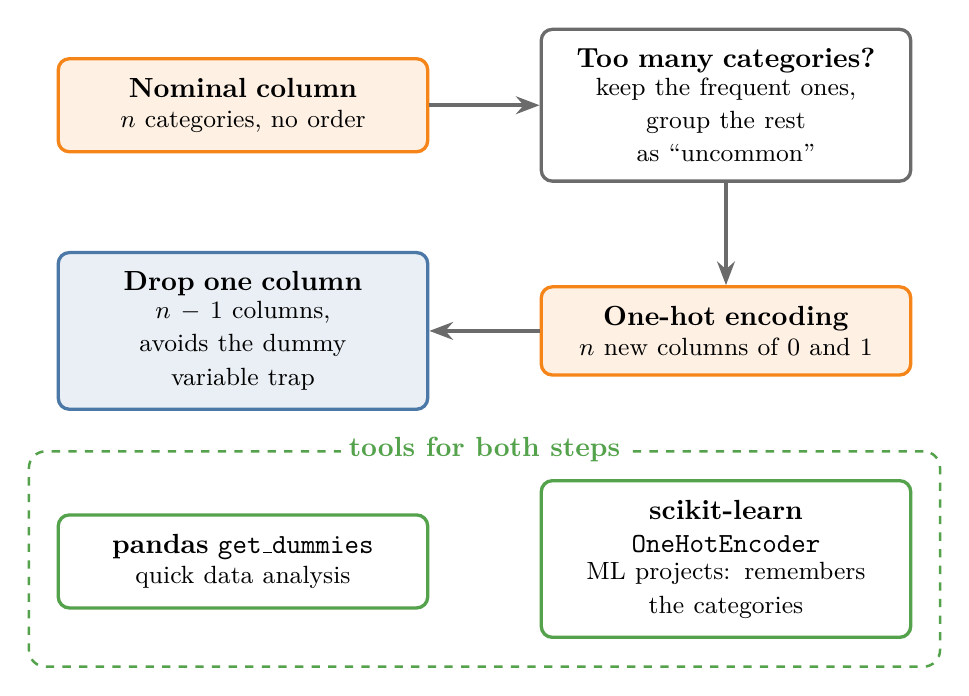
\begin{tikzpicture}[node distance=1.2cm]
  \node[box=corange, text width=4.2cm] (nom) {\textbf{Nominal column}\\[-1pt]\small $n$ categories, no order};
  \node[box=cgrey, fill=white, text width=4.2cm, right=1.4cm of nom] (many) {\textbf{Too many categories?}\\[-1pt]\small keep the frequent ones,\\ group the rest as ``uncommon''};
  \node[box=corange, text width=4.2cm, below=1.3cm of many] (ohe) {\textbf{One-hot encoding}\\[-1pt]\small $n$ new columns of 0 and 1};
  \node[box=cblue, text width=4.2cm, left=1.4cm of ohe] (drop) {\textbf{Drop one column}\\[-1pt]\small $n-1$ columns,\\ avoids the dummy variable trap};
  \draw[arrow] (nom) -- (many);
  \draw[arrow] (many) -- (ohe);
  \draw[arrow] (ohe) -- (drop);
  \node[box=cgreen, fill=white, text width=4.2cm, below=1.3cm of drop] (pd) {\textbf{pandas} \texttt{get\_dummies}\\[-1pt]\small quick data analysis};
  \node[box=cgreen, fill=white, text width=4.2cm, below=1.3cm of ohe] (sk) {\textbf{scikit-learn} \texttt{OneHotEncoder}\\[-1pt]\small ML projects: remembers\\ the categories};
  \begin{scope}[on background layer]
    \node[draw=cgreen, dashed, rounded corners=6pt, line width=0.9pt, inner sep=10pt, fit=(pd)(sk)] (tools) {};
  \end{scope}
  \node[font=\sffamily\bfseries, text=cgreen, fill=white, inner sep=3pt] at (tools.north) {tools for both steps};
\end{tikzpicture}
\end{document}
